%\documentclass[aps,prl,twocolumn,showpacs,superscriptaddress,groupedaddress]{revtex4}  % for review and submission
%\documentclass[aps,preprint,showpacs,superscriptaddress,groupedaddress]{revtex4}  % for double-spaced preprint
\documentclass[aps,prl,floatfix,twocolumn,10pt]{revtex4-1}  % for review and submission
%\documentclass[aps,prl,preprint]{revtex4-1}  % for double-spaced preprint
\usepackage{graphicx}  % needed for figures
\usepackage{subfigure} % for subfigures
%\usepackage{dcolumn}   % needed for some tables
%\usepackage{bm}        % for math
\usepackage{amssymb}   % for math
\usepackage{upgreek}	% for non-italic greek letters
	
% avoids incorrect hyphenation, added Nov/08 by SSR
\hyphenation{ALPGEN}
\hyphenation{EVTGEN}
\hyphenation{PYTHIA}

%% New commands
\newcommand{\unit}[1]{\ensuremath{\, \mathrm{#1}}}
\newcommand{\msub}[1]{\ensuremath{\textnormal{\begin{tiny}#1\end{tiny}}}}


\begin{document}

\title{Compact X-ray grating interferometry at 100~keV}

\author{T.~Thuering}
  \affiliation{Paul Scherrer Institut, Villigen PSI, Switzerland}
  \affiliation{Institute for Biomedical Engineering, Swiss Federal Institute of Technology, Zurich, Switzerland}
\author{M.~Abis}
  \affiliation{Paul Scherrer Institut, Villigen PSI, Switzerland}
  \affiliation{Institute for Biomedical Engineering, Swiss Federal Institute of Technology, Zurich, Switzerland}
\author{Z.~Wang}
  \affiliation{Paul Scherrer Institut, Villigen PSI, Switzerland}
\author{C.~David}
  \affiliation{Paul Scherrer Institut, Villigen PSI, Switzerland}
\author{M.~Stampanoni}
  \affiliation{Paul Scherrer Institut, Villigen PSI, Switzerland}
  \affiliation{Institute for Biomedical Engineering, Swiss Federal Institute of Technology, Zurich, Switzerland}

\date{\today}


\begin{abstract}
Todays X-ray phase contrast imaging techniques are not only limited by spatial and temporal coherence properties of the beam, but also in the applicable energy range due to technical limitations. Imaging at higher energies is of particularly high interest as it would clearly expand the range of applications, e.g., towards the examination of materials with a higher density or thickness. Grating interferometry, albeit proven to be one of the most promising methods for the industrial applicability, is limited to energies up to about $50 \unit{keV}$ by the fabrication of gratings with sufficiently high aspect ratios. Here, we propose an alternative approach, which enables the access to the entire diagnostic energy range of X-rays for phase and dark field contrast imaging on compact systems with low brilliance X-ray tubes. Based on Talbot-Lau interferometry, the novel approach involves the edge-on illumination of specially designed gratings, which solves two fundamental problems. First, the effective aspect ratio is not determined or limited by the structure height limitation of the manufacturing technology and thus, arbitrary aspect ratios are feasible. Secondly, the intrinsic reduction of the field of view for higher aspec ratios is solved by a circular alignment of the grating structures. Based on this, a compact Talbot-Lau interferometer has been set up with a design energy at $100 \unit{keV}$, providing 2D and 3D phase contrast images of dense materials. The approach is not only applicable to X-rays, but is also compatible to other grating based imaging modalities such as neutrons.
\end{abstract}

%\pacs{}
\maketitle

%%%%%%%%%%%%%%%%%%%%%%%%%%%%%%%%%%%%%%%%%%%%%%%%%%%%%%%%%%%%%%%%%%%%%%%%
% Body of paper
%%%%%%%%%%%%%%%%%%%%%%%%%%%%%%%%%%%%%%%%%%%%%%%%%%%%%%%%%%%%%%%%%%%%%%%%


%Introduction
X-ray radiography and computed tomography (CT) are nowadays standard imaging techniques for non-destructive testing of materials or for medical diagnosis in daily routine. The physical contrast mechanism relies on the attenuation of X-rays in an object through the photo-electric effect or Compton scattering, whereas two materials can be distinguished due to their different attenuation properties. The wave and particle nature of X-rays reveal two further physical interaction mechanisms that occur if an object is exposed to X-rays.

Regarding the wave properties, an interface of two different materials in an object causes a change in the wave's phase velocity and thus in a net change of the output phase (a phase shift) downstream of the object. Since no detection device is able to measure a phase shift directly, advanced techniques are necessary to obtain access to this signal.

Regarding the particle properties of X-rays, photons are randomly scattered on small structures in the material. Depending on the imaging system (geometry and energy), wide angle and small angle scattering represent typical sources of noise in absorption imaging. For the type of scattering which occurs exclusively in forward direction and under ultra small angles (order of nano radiants), the particles usually remain within the area of a detector pixel and thus this effect cannot directly be detected.

The main interest in the detectability of those additional interaction mechanisms is the fact that attenuation, phase shift and scattering are phyiscally complementary interaction mechanisms, in the sense that their occurence is mutually independent. In the context of information content of images, this gives rise to hypothesize that the complementary interaction mechanisms may eventually yield complementary image information, manifested with different image contrasts.

Since currently available phase contrast techniques rely on secondary physical effects, such as interference, and thus typically on optical hardware (e.g. crystals, gratings), they vary a lot in terms of sensitivity, practical applicability or achievable resolution. The vast majority of the methods, including crystal analyzer based \cite{Davis1995,Chapman1997} or interferometric \cite{Bonse1965,Momose1996} methods rely on X-ray beams of high spatial and temporal coherence, available only at synchrotons. Techniques with a high degree of spectral acceptance are inline phase contrast \cite{Snigirev1995,Wilkins1996,Cloetens1996} and Talbot interferometry \cite{Cloetens1997,David2002,Momose2003a}. Regarding the acceptance of X-ray beams with low temporal and spatial coherence, Talbot-Lau interferometry \cite{Pfeiffer2006} and coded apertures \cite{Munro2012} are currently the only feasible techniques.

While current phase contrast methods are today broadly available on synchrotrons and constantly improving for conventional X-ray tubes, the applicable energy range is still limited to the low energy range. All of the reported methods have been designed for X-ray energies between 5 and 40 keV. None of the current methods is compatible to industrial or medical applications, where higher X-ray energies ($>50 \unit{keV}$) are required. For instance, the portability of Talbot-Lau interferometry towards medical imaging such as chest or abdominal radiography or CT, which require energies up to $150 \unit{keV}$, has still been impossible due to the technical limitations in grating fabrication for X-ray energies higher than approx. $50 \unit{keV}$. Grating manufacturing methods are well established for energies up to about $E=40 \unit{keV}$, which partly explains the reported successes of the technique in mammography \cite{Stampanoni2011} or hand imaging \cite{Thuering2013a}. The limiting factor for currently available grating fabrication techniques is the aspect ratio $\textnormal{AR} = 2h/p$, where $p$ is the grating period and $h$ the structure height. For a given setup distance, $p \propto 1/\sqrt{E}$ and $h \propto E^3$, and for the aspect ratio, it can be shown that $\textnormal{AR} \propto E^{7/2}$. While for $25 \unit{keV}$, an aspect ratio for the absorption grating of around $\textnormal{AR}=30$ is necessary for a reasonable setup length, it would have to be at least 128 for $100 \unit{keV}$. This is only approximate and ignores absorption edges of the materials (e.g., at around $80 \unit{keV}$ for gold in an absorption grating). Furthermore, when using a polychromatic spectrum, photons above the design energy should also be efficiently attenuated by the gratings to guarantee their contribution to the signal, requiring even higher aspect ratios. The current technical limitation is at $\textnormal{AR} \approx 50$, whereas such high values are pushing the limits and usually come at the expense of a poor grating quality and performance.






% Grating interferometry is currently the most promising technique to become a widespread method for multimodal imaging using phase and scattering contrast.
% 
% Grating interferometry exploits the Talbot effect of a periodic phase grating (beam splitter) to generate an interference pattern, which can then be sensed for any changes in intensity (absorption signal), lateral shift \cite{David2002} (refraction signal) and amplitude \cite{Pfeiffer2008} (scattering signal) by using an analyzer grating (absorption grating) \cite{Momose2003a}. The compatibility to standard low-brilliance X-ray sources, being the most valuable property in terms of practical applicability, is on one hand achieved with a third grating in front of the source (source grating) \cite{Pfeiffer2006}. On the other hand, the comparably high degree of achromaticity of a grating interferometer enables the operation with the polychromatic spectrum.
% 
% In the past few years, the potential impact of grating interferometry on conventional X-ray tubes has been studied for a variety of applications in medical imaging or materials science, whereas the most prominent contributions in the medical field are probably from mammography \cite{Stampanoni2011} or from human hand imaging \cite{Donath2010a,Thuering2013}. *** anyhting from the pfeiffer group? *** 
% 
% The portability of this technique towards medical applications such as chest or abdominal radiography or CT has so far been difficult due to the requirement of higher X-ray energies (up to $150 \unit{keV}$). Gratings with reliable quality can be fabricated for energies up to about $E=40 \unit{keV}$, which partly explains the success of the technique in mammography or hand imaging. The limiting factor of currently available grating fabrication techniques is the aspect ratio, given by $\textnormal{AR} = 2h/p$, where $p$ is the grating period and $h$ the structure height. For a given setup distance, $p \propto 1/\sqrt{E}$ and $h \propto E^3$, such that for the aspect ratio, we obtain $\textnormal{AR} \propto E^{7/2}$. While for $25 \unit{keV}$, an aspect ratio for the absorption grating of around $\textnormal{AR}=30$ is necessary for a reasonable setup length, it would have to be $\textnormal{AR} \approx 128$ for $100 \unit{keV}$. This rough calculation is only approximate and ignores absorption edges of the materials (e.g., at around $80 \unit{keV}$ for gold in an absorption grating). Furthermore, when using a polychromatic spectrum, photons above the design energy should also be efficiently attenuated by the gratings to guarantee their contribution to the signal, requiring even higher aspect ratios.

We herein propose an alternative design method of X-ray Talbot-Lau grating interferometers, which allows phase contrast and dark field imaging with low brilliance X-ray tubes at arbitrarily high energies. The approach is based on the edge-on illumination of gratings. Edge-on illumination, as opposed to the standard face-on illumination, exploits the arbitrary length of the grating lines to form high aspect ratios of the structures along the beam direction. Since the effective structure height of the grating is in then determined by the grating dimension, the aspect ratio can be arbitrarily high. FIG.~\ref{Fig:schematic} illustrates the edge-on illumination approach.

%We herein propose an alternative design method of X-ray grating interferometry, which allows phase and dark field imaging at arbitrarily high energies. The approach is based on the edge-on illumination of gratings. Edge-on illumination, as opposed to the standard face-on illumination, has the advantage that the dimension along the grating lines, which originally has been the vertical dimension in the image plane, is now the dimension defining the effective structure height $h_\msub{eff}$ of the grating in beam direction. Since this dimension is only limited by the achievable grating size, the effective aspect ratio $\textnormal{AR}_\msub{eff}$ can virtually be of any size. 
\begin{figure} [ht]
  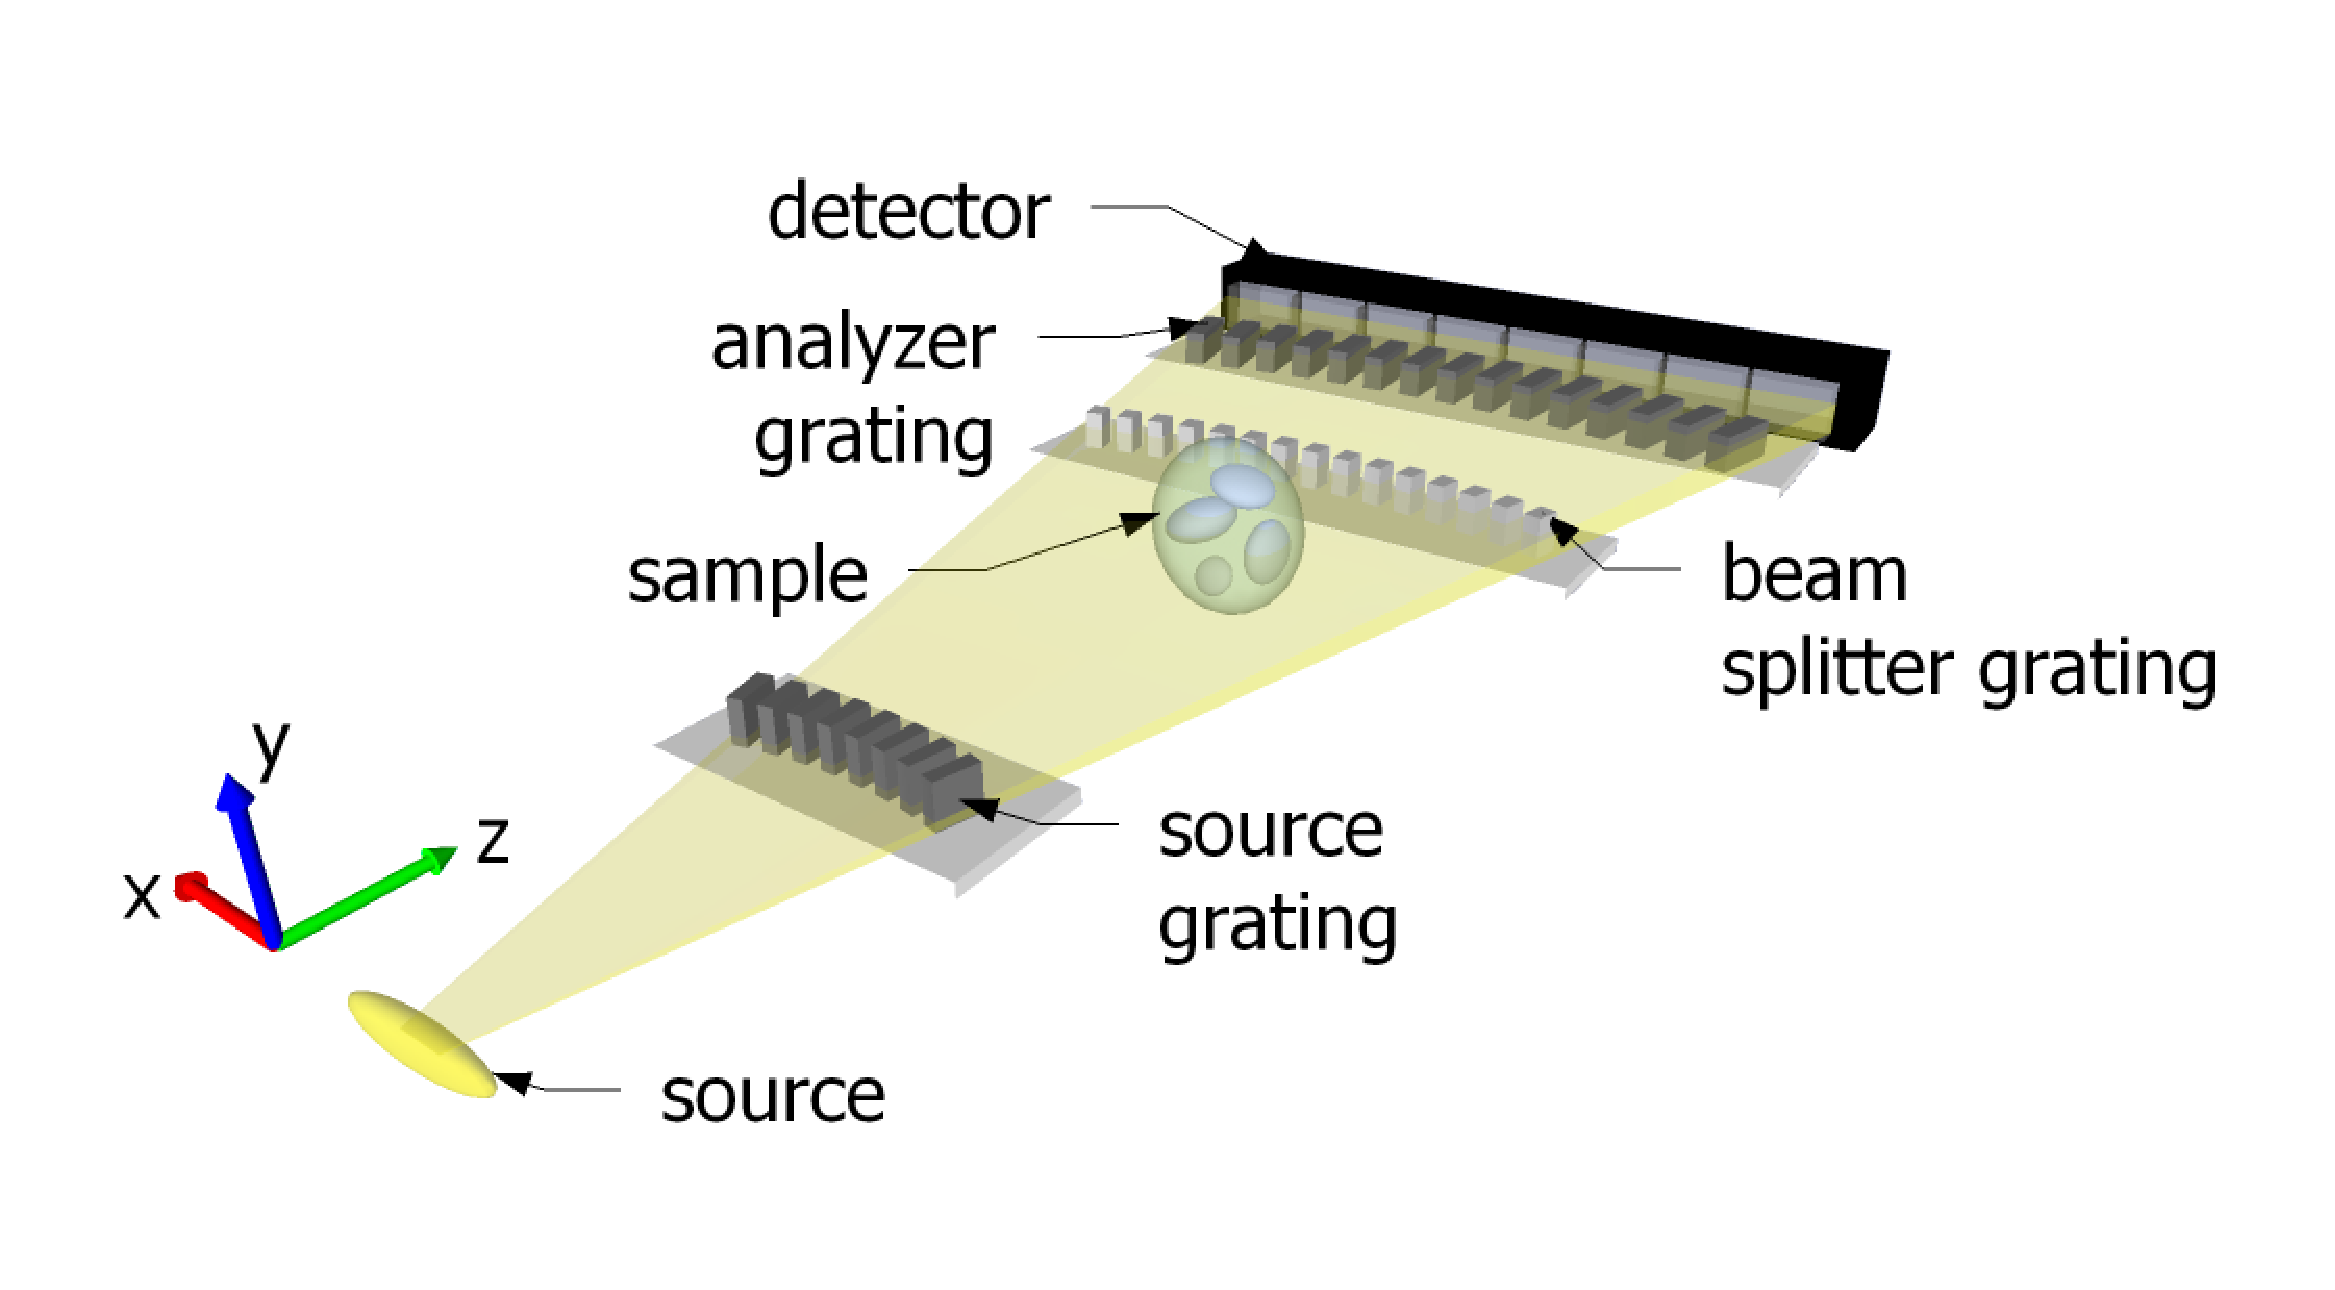
\includegraphics[width = \linewidth]{figures/figure1.eps}
  \caption{Schematic of a grating interferometer for high X-ray energies in edge-on illumination mode. The gratings are curved to maintain a large field of view.}
  \label{Fig:schematic}
\end{figure}

Increasing the effective aspect ratio of the gratings typically leads to a reduction of the field of view due to the change of the transmission function at high incident angles, which has also been demonstrated by using a glancing angle of the gratings between zero and $90$ degrees \cite{Stutman2012}. In order to overcome this problem in edge-on illuminated grating interferometry, the grating lines are alined on an arc with a radius equal to the distance from the source to the grating.

The combination of edge-on illumination and the circularly curved structure alignment allows to design a grating interferometer at any design energy in the diagnostic energy range of X-rays. The arbitrary aspect ratio only comes at the expense of a limited field of view in the vertical dimension of the image plane, which is, depending on the detector, typically a few pixels. However, radiographic 2D images can still be acquired in scanning mode without increasing dose. Similary, in tomographic mode, the approach allows single slice CT or full 3D imaging in scanning mode.

%A similar approach to increase the effective aspect ratios has successfully been demonstrated by using a glancing angle of the gratings between zero and $90$ degrees \cite{Stutman2012}. With this approach, conventional gratings mounted on a rotation stage can be used, keeping the grating design simple and standard. However, a major limitation of this method is the severe reduction of the field of view at higher glancing angles, due to the non-curved alignment of the grating structures.

Gratings were manufactured by Micro Works GmbH, Germany, using a LIGA process \cite{Kenntner2010}. The grating design and fabrication is non-standard and involves a complex mask design, as shown in FIG. 2. Each grating is on a $5 \times 60 \unit{mm^2}$ silicon chip and has its specific structure length and curvature. Several grating chips can be fabricated on a single 4 inch silicon wafer. For the present experiments, a symmetric interferometer with a grating period of $p = 2.8 \unit{\upmu m}$ has been used. The design energy is $100 \unit{keV}$ and the beam splitter grating periodically shifts the phase by zero and $\pi$ at this energy. Using gold as the phase shifting material, this requires a structure length of $b = 19.8 \unit{\upmu m}$. The analyzer grating is an absorption mask for sensing the changes of the interference pattern generated by the beam splitter. The structure length of this grating is $b = 800 \unit{\upmu m}$, providing sufficient attenuation of the X-rays up to $160 \unit{keV}$. Beam splitter- and analyzer grating are separated at the first fractional Talbot order and the distance from the source grating to the analyzer grating is $32 \unit{cm}$.

The X-ray source is a COMET MXR-160HP/11 X-ray tube with a maximum output voltage of $160 \unit{kV}$. Since the absorption gratings perform efficiently up to $160 \unit{keV}$ and the spectral acceptance at the first fractional Talbot order is high (50 to $>160 \unit{keV}$), the tube voltage was set to the maximum of $160 \unit{kV}$ and operated at a current of $10 \unit{mA}$. The focal spot size is approx. $1 \unit{mm}$. The detector is a CCD camera from Finger Lakes Instruments. A cesium idodide (CsI) scintillator of $600 \unit{\upmu m}$ thickness converts the X-rays to visible light and is coupled with an optical lens projecting the image onto the CCD. The effective pixel size is $80 \unit{\upmu m}$. With a grating structure height of approx. $100 \unit{\upmu m}$, the field of view in the vertical direction is limited to one pixel row. In addition to the standard components (source, camera, interferometer), two optical slit, one in front of the source grating, the other in front of the camera, have been installed for the collimation of the beam in vertical direction. X-rays which are not travelling through all of the gratings do not contribute to the signal and must be attenuated by the slits. The slit widths are $25 \unit{\upmu m}$ and $100 \unit{\upmu m}$, respectively.

FIG. 3 shows a radiographic image of a metal screw in all three contrast modes, acquired with the $100 \unit{keV}$ grating interferometer setup. Grating interferometry at such a high diagnostic energy allows to examine more dense materials such as heavy metals in phase contrast mode. At lower energies, the phase shifts would be too large and wrap over multiple periods of the analyzer grating.


We thank Gordan Mikuljan from Paul Scherrer Institute, Switzerland, for his work on the mechanical design, Joachim Schulz and Marco Walter from Micro Works GmbH, Germany, for the competent support on grating design issues, Christian Kottler and Vincent Revol from Centre Suisse d'Electronique et de Microtechnique (CSEM), Switzerland for the fruitful discussions on grating interferometer design.






%If the spatial coherence of the beam is too low to form interference, another absorption grating, splitting the beam into an array of smaller sources, can be added.Adding another absorption grating in front of a



%In wave optics, the two interaction mechanisms of X-ray with matter are described by the complex index of refraction, $n=1-\dleta  + i\beta$, where $\beta$ takes into account the absorption and $\delta$ the phase shift properties of the material.
 



- Grating interferometry can yield additional information. bla bla

- Signal decay of the attenuation coefficient $\mu$ is proportional to $1/E^3$, for phase it is only $1/E$. -> Higher benefit of PC at higher energies. optimum energy (according to raupach paper) of PC compared to ABS is .... (figure out from raupach paper or so).

- high energies are important for thick samples and medical CT applications

- grating interferometry is the most promising technique for PC on conventional X-ray tubes. It further allows to retrieve a dark field image. So far, grating interferometry was limited in field of view and energy. High aspect ratios are essential for grating interferometry at high energies. Glancing angle has been reported and increased the aspect ratio and thus visibility \cite{Stutman2012}. However, the problem of a reduced field of view (reported as vignetting in Stutman) becomes severe for low glancing angles. So, higher aspect ratios always reduce the field of view.

- Here, a new method by using curved gratings in edge illumination mode, is presented. Description of edge illumination principle: tilting the grating in 90 degrees, the limiting dimension is now the vertical axis, radiography is possible only in scanning mode, single slice tomography is possible. High field of view by curved gratings, curved gratings represent an elegant solution to the limited FOV, which has already been demonstrated for compact grating interferometery \cite{Thuering2011}.

%Methods
- Setup basic hardware: The X-ray source is a COMET MXR-160HP/11 X-ray tube with a maximum output voltage of $160 \unit{kV}$. The detector consists of a cesium idodide (CsI) scintillator of $600 \unit{\mu m}$ thickness, an optical lens and a CCD camera from Finger Lakes Instruments. The effective pixel size is $80 \unit{\mu m}$. 

- Grating manufacturing: 

- setup design: Due to the large focal spot size of the source of approx. $1 \unit{mm}$, the grating interferometer is a Talbot-Lau type interferometer with a source grating \cite{Pfeiffer2006}. Symmetric design, $p_0 = p_1 = p_2 = 2.8 \unit{\mu m}$. Design energy at ... keV, Talbot order .... Gold was used for the absorption grating. The effective thickness of the gold structure in beam direction is $800 \unit{\mu m}$, resulting in an aspect ratio of $2h/p \approx 570$. For the phase shifting grating, Nickel/Gold with a thickness of $... \unit{\mu m}$, generating a phase shift of $\pi$ at the design energy. The vertical FOV is limited by the height of the grating structures of G2, which is $100 \unit{\mu m}$. With a pixel size of $80 \unit{\mu m}$, only a single detector line must be read out. To avoid blurring of the interference pattern in perpendicular direction of this line, an efficient beam collimation has been implemented. Two collimator slits have been used, one with a slit height of $25 \unit{\mu m}$ placed after the source and another one with a slit width of $100 \unit{\mu m}$ placed between G2 and the detector.


%Results
- It would be nice to show an image from the slit, where also the fringes are visible. Specify visibility \\
- Phantom tomography \\
- Real data tomography \\
- Effect of scattering (Silvia) \\







\bibliography{library.bib}
\bibliographystyle{apsrev4-1}

\end{document}